\section{Preliminary} \label{sec.preliminary}

\begin{figure}[h!]
\centering
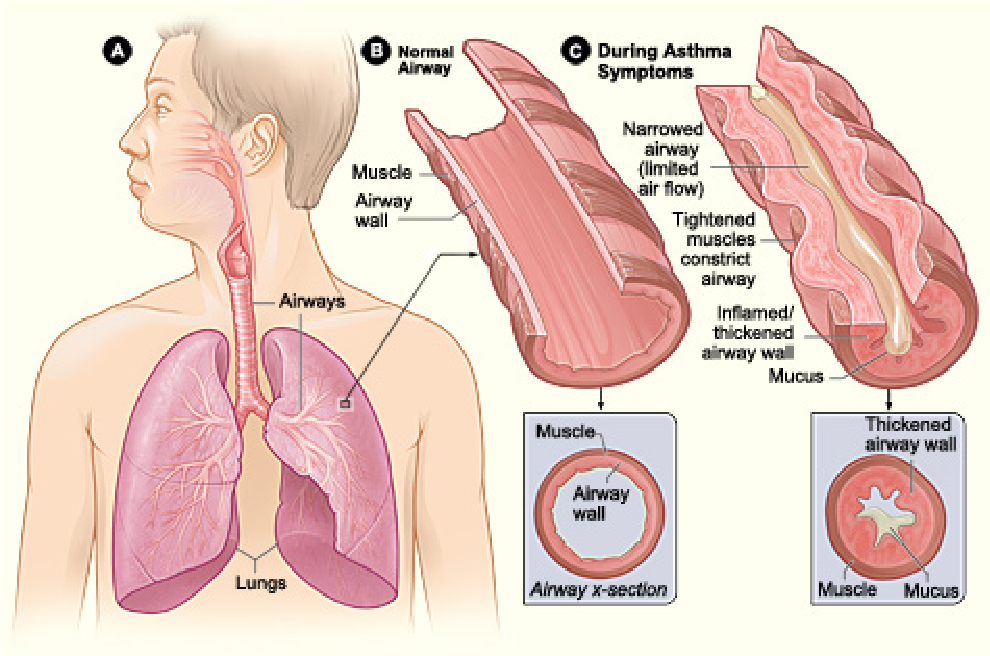
\includegraphics[width=0.36\textwidth]{Aasthma.pdf}
\caption{Concept diagram of asthma formation~\cite{NH}}
\label{fig.Asthma}
\end{figure}
Figure~\ref{fig.Asthma} shows how the airway narrows when asthma attack occurs. Airways are tubes that carry air into and out of our lungs. People who have asthma attack experience usually have inflamed airways. When the airways respond to triggers, the muscles around the airways will tighten. In addition, mucus is a sticky, thick liquid that can further make the airways narrow and narrowed airways allow less air to flow into lungs. As a result, asthma symptoms may occur, such as recurring periods of wheezing (a whistling sound when you breathe), chest tightness, shortness of breath, and coughing.

The breathing activity is performed primarily by the diaphragm, a large muscle that separates the thoracic cavity from the abdominal cavity. During inspiration (breathing in), diaphragm contracts, draws downward, and creates a vacuum in thoracic cavity. This vacuum inflates lungs by drawing air into body through the trachea or windpipe. During normal expiration (breathing out), the diaphragm relaxes and allows air to flow out as the lungs deflate, similar to the way that an inflated balloon deflates when releases. When people have asthma attack, their respiratory pattern changes and the movement pattern of diaphragm also changes.

Ultrasound is a non-invasive and real-time tool used for imaging soft tissues. Medical ultrasound is based on the use of high frequency sound to aid in diagnosis and treatment of patients. Usually, ultrasound frequencies range from 2 to 15 MHz approximately. Ultrasound waves (pulses of sound) are emitted from a transducer, propagate through different tissues, and return to the transducer as reflected echoes. Ultrasound is conducted with different speeds in a various of body tissues. Some tissues absorb sound waves while others reflect them. The density of the tissues corresponds to the speed at which the echoes return. There are different ways to visualize the obtained ultrasound information, which are called ultrasound modalities. The most common modes are A-mode, B-mode, and M-mode. The 'A' in A-mode stands for Amplitude. Information of the reflected signal in a single ultrasound beam is continually displayed. Distance from the transducer and signal intensity are shown by position and amplitude as a line on an oscilloscope. This mode is mainly used for historical interest. The 'B' in B-mode stands for Brightness. B-mode information can form a sector in a plane of the body, shown as pixel intensity on a monitor. In B-mode ultrasound image, fluid is black, tissue is gray, and bone is white. The denser the tissue is, the brighter white it appears. The brightest white is bone. B-mode often generates 2D image, which  is the most important modality for anatomic assessment and orientation in the body. The 'M' in M-mode stands for Motion. This represents movement of ROI over time. The M-mode has good temporal resolution, so that it is useful in detecting and recording rapid movements. In this paper, the goal is to locate the diaphragm region in ultrasound image. For this reason, we choose the B-mode to collect data as Youngkyoo suggested~\cite{hwang2012robust}.


